 \documentclass[11pt]{article}

\usepackage{latexsym}
\usepackage{amssymb}
\usepackage{amsthm}
\usepackage{amscd}
\usepackage{amsmath}
\usepackage{tikz}
\usepackage{graphicx}
\usepackage{enumerate}
\usepackage[final]{pdfpages}


\newcommand{\ZZ}{\mathbb{Z}}

\setlength{\evensidemargin}{1in}
\addtolength{\evensidemargin}{-1in}
\setlength{\oddsidemargin}{1.5in}
\addtolength{\oddsidemargin}{-1.5in}
\setlength{\topmargin}{1in}
\addtolength{\topmargin}{-1.5in}

\setlength{\textwidth}{16cm}
\setlength{\textheight}{23cm}

\newcommand{\rook}{\hspace{-.1cm}\amalg\hspace{-.15cm}\bar{}}
\newcommand{\Stab}{\mathrm{Stab}}
\newcommand{\FF}{\mathbb{F}}


\begin{document}
\begin{center}
\section*{William Daniels}
\section*{CSCI 4630}
\subsection*{Linguistic Geometry}
\subsection*{Homework \#7 03/16/15}
\end{center}

\vspace{.25cm}

First, the zone in question is shown below (just using the main trajectory as specified in the problem, instead of the white bishop going 'left' first): \\\\
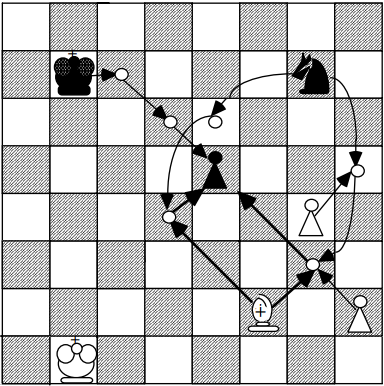
\includegraphics{P1Zone.png}\\\\

Now, to analyze the motion of a few pices on the board (we'll do 3 of them).
\begin{enumerate}
\item The first set of moves we'll consider starts with the main trajectory:
\begin{enumerate}[(a)]
\item Translation: $B_1 = TRANSITION(BISHOP, f7, g6)$ , this causes the following to happen: 
$$\Pi_{B_1}(t_B) \text{ is a shortened trajectory with excluded first symbol, i.e. }$$
$$\Pi_{B_1}(t_B) = t_{B,s} = a(g6)a(e4)$$
both trajectories of the black knight ($BKN_1, BKN_2$) should be dropped, since the black knight no longer has enough time to reach the white bishop, and the secondary bishop trajectory got dropped. This also drops the negation trajectory of the WPAWN1, since the Black knight trajectory is no longer there. The negation trajectory of the WPAWN2 also gets dropped because you can't have a negation trajectory that aims directly at a new piece. 
All other trajectories are unaffected. \\
\item With the previous move in consideration, the next move could be $TANSITION(BKING, b2, c2)$ which would have a similar result: 
$$\Pi_{BK_1}(t_BK) \text{ is a shortened trajectory with excluded first symbol, i.e. }$$
$$\Pi_{BK_1}(t_BK) = t_{B,s} = a(d3)a(e4)$$
no other trajectories are affected. \\
\end{enumerate}
\item Now lets try a different set of moves:
\begin{enumerate}[(a)]
\item The first move will be $ TRANSITION(WPAWN1, g5, g4)$\\
This actually results in the entire dropping of all trajectories of the white pawn 1, no other trajectories are effected.
\end{enumerate}
\item for the final translation, we'll start with the bishop again, but show a capture instead. 
\begin{enumerate}[(a)]
\item  The first move is the same as the first set of moves: Translation: $B_1 = TRANSITION(BISHOP, f7, g6)$ , this causes the following to happen: 
$$\Pi_{B_1}(t_B) \text{ is a shortened trajectory with excluded first symbol, i.e. }$$
$$\Pi_{B_1}(t_B) = t_{B,s} = a(g6)a(e4)$$
both trajectories of the black knight ($BKN_1, BKN_2$) should be dropped, since the black knight no longer has enough time to reach the white bishop, and the secondary bishop trajectory got dropped. This also drops the negation trajectory of the WPAWN1, since the Black knight trajectory is no longer there.  The negation trajectory of the WPAWN2 also gets dropped because you can't have a negation trajectory that aims directly at a new piece. 
All other trajectories are unaffected. \\
\item now, there are really only two moves left to the black pieces, and since we've already considered the black king, lets consider the black pawn 1: $TRANSITION(BPAWN1, e5, e6)$
Now, since this deletes the primary trajectory, the entire zone must be regenerated. 
\end{enumerate}
\end{enumerate}

Now, for the second problem, the zone looks like the following: \\
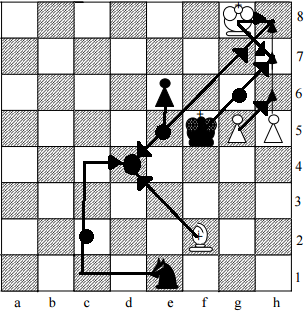
\includegraphics{P2Zone.png}\\\\


The table that represents the motion is on the following page: 

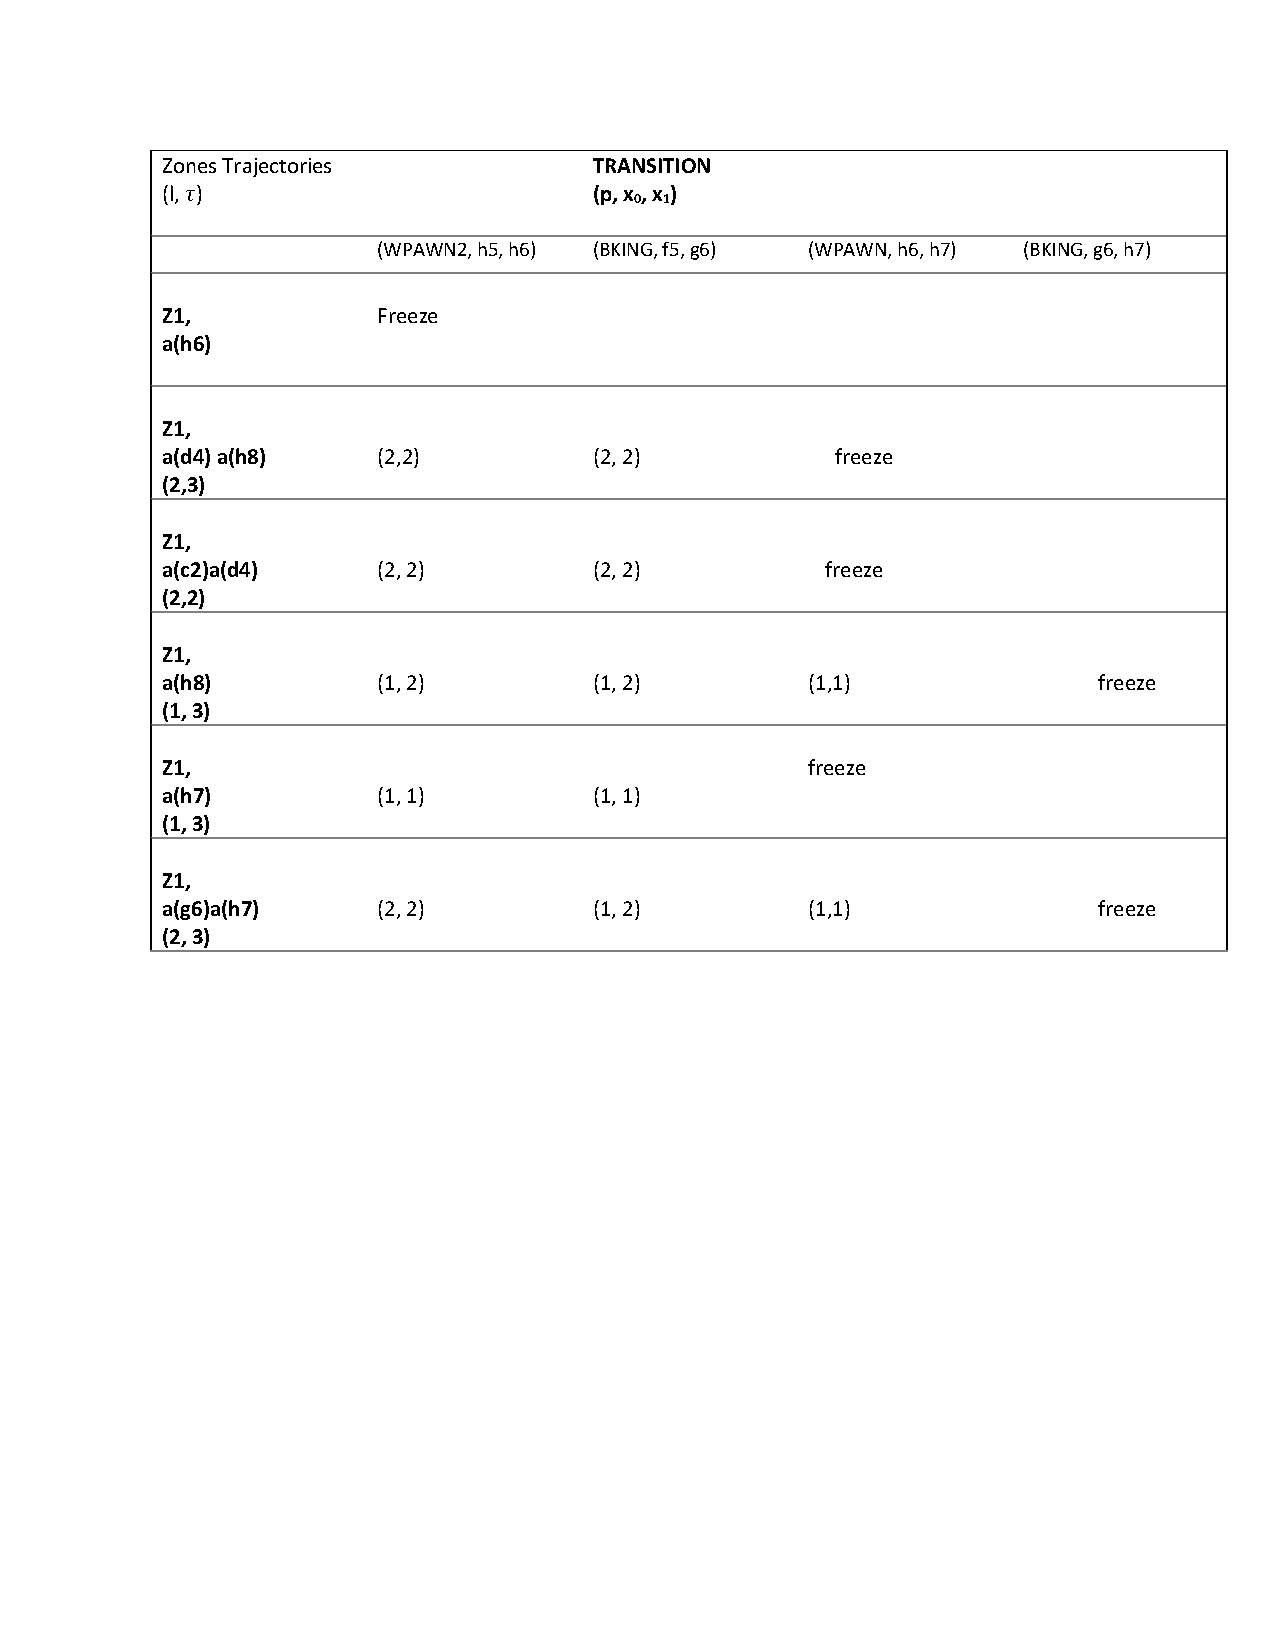
\includepdf[pages=1]{ZoneTable.pdf}





\end{document}

